\begin{figure}[ht]
\centering
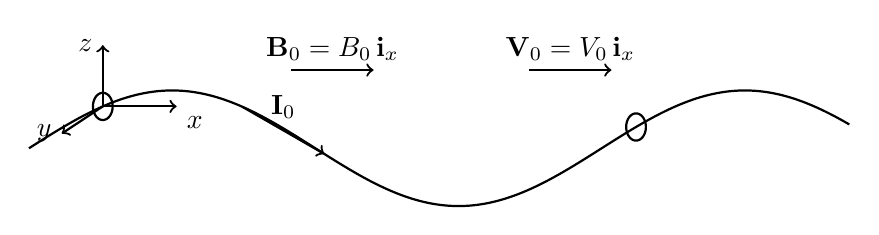
\begin{tikzpicture}

\begin{axis}[
  width=12cm,
  height=4cm,
  axis lines=none,
  xmin=0, xmax=10,
  ymin=-1.4, ymax=1.4,
  clip=false
]

% Wavy string
\addplot[thick, smooth, samples=200, domain=0:10]
  {0.85*sin(deg(0.9*x))};

% --- Define left loop location ---
\pgfmathsetmacro{\xloop}{0.9}
\pgfmathsetmacro{\yloop}{0.85*sin(deg(0.9*\xloop))}

% Precompute axis-coordinate endpoints for the triad
\pgfmathsetmacro{\xplus}{\xloop + 0.9}
\pgfmathsetmacro{\xminus}{\xloop - 0.5}
\pgfmathsetmacro{\yminus}{\yloop - 0.4}
\pgfmathsetmacro{\yplus}{\yloop + 0.9}

% --- Coordinate triad attached to left loop ---
\draw[->,thick] (axis cs:\xloop,\yloop) -- (axis cs:\xplus,\yloop)
  node[below right] {$x$};
\draw[->,thick] (axis cs:\xloop,\yloop) -- (axis cs:\xminus,\yminus)
  node[left] {$y$};
\draw[->,thick] (axis cs:\xloop,\yloop) -- (axis cs:\xloop,\yplus)
  node[left] {$z$};

% --- Left loop ---
\addplot[thick, domain=0:360, samples=100]
  ({\xloop + 0.12*cos(x)}, {\yloop + 0.20*sin(x)});

% --- Right loop (new) ---
\pgfmathsetmacro{\xloopR}{7.4}
\pgfmathsetmacro{\yloopR}{0.85*sin(deg(0.9*\xloopR))}
\addplot[thick, domain=0:360, samples=100]
  ({\xloopR + 0.12*cos(x)}, {\yloopR + 0.20*sin(x)});

% B0 arrow
\draw[->,thick] (axis cs:3.2,1.15) -- (axis cs:4.2,1.15);
\node[above] at (axis cs:3.7,1.15) {$\mathbf{B}_0 = B_0\,\mathbf{i}_x$};

% V0 arrow
\draw[->,thick] (axis cs:6.1,1.15) -- (axis cs:7.1,1.15);
\node[above] at (axis cs:6.6,1.15) {$\mathbf{V}_0 = V_0\,\mathbf{i}_x$};
% --- Current arrow along the string + label on the string (new) ---
% Pick two x-positions along the curve and compute y from the same function
\pgfmathsetmacro{\xIstart}{2.6}
\pgfmathsetmacro{\yIstart}{0.85*sin(deg(0.9*\xIstart))}
\pgfmathsetmacro{\xIend}{3.6}
\pgfmathsetmacro{\yIend}{0.85*sin(deg(0.9*\xIend))}
\pgfmathsetmacro{\xImid}{0.5*(\xIstart+\xIend)}
\pgfmathsetmacro{\yImid}{0.85*sin(deg(0.9*\xImid))}

% Arrow (direction: start -> end)
\draw[->,thick] (axis cs:\xIstart,\yIstart) -- (axis cs:\xIend,\yIend);

% Label placed on/near the curve
\node[above] at (axis cs:\xImid,\yImid) {$\textbf{I}_0$};

\end{axis}
\end{tikzpicture}
\caption{Schematic of the string with the applied fields and forces.}
\label{fig:string_schematic}
\end{figure}
